\documentclass[twoside]{book}

% Packages required by doxygen
\usepackage{fixltx2e}
\usepackage{calc}
\usepackage{doxygen}
\usepackage{graphicx}
\usepackage[utf8]{inputenc}
\usepackage{makeidx}
\usepackage{multicol}
\usepackage{multirow}
\PassOptionsToPackage{warn}{textcomp}
\usepackage{textcomp}
\usepackage[nointegrals]{wasysym}
\usepackage[table]{xcolor}

% Font selection
\usepackage[T1]{fontenc}
\usepackage{mathptmx}
\usepackage[scaled=.90]{helvet}
\usepackage{courier}
\usepackage{amssymb}
\usepackage{sectsty}
\renewcommand{\familydefault}{\sfdefault}
\allsectionsfont{%
  \fontseries{bc}\selectfont%
  \color{darkgray}%
}
\renewcommand{\DoxyLabelFont}{%
  \fontseries{bc}\selectfont%
  \color{darkgray}%
}
\newcommand{\+}{\discretionary{\mbox{\scriptsize$\hookleftarrow$}}{}{}}

% Page & text layout
\usepackage{geometry}
\geometry{%
  a4paper,%
  top=2.5cm,%
  bottom=2.5cm,%
  left=2.5cm,%
  right=2.5cm%
}
\tolerance=750
\hfuzz=15pt
\hbadness=750
\setlength{\emergencystretch}{15pt}
\setlength{\parindent}{0cm}
\setlength{\parskip}{0.2cm}
\makeatletter
\renewcommand{\paragraph}{%
  \@startsection{paragraph}{4}{0ex}{-1.0ex}{1.0ex}{%
    \normalfont\normalsize\bfseries\SS@parafont%
  }%
}
\renewcommand{\subparagraph}{%
  \@startsection{subparagraph}{5}{0ex}{-1.0ex}{1.0ex}{%
    \normalfont\normalsize\bfseries\SS@subparafont%
  }%
}
\makeatother

% Headers & footers
\usepackage{fancyhdr}
\pagestyle{fancyplain}
\fancyhead[LE]{\fancyplain{}{\bfseries\thepage}}
\fancyhead[CE]{\fancyplain{}{}}
\fancyhead[RE]{\fancyplain{}{\bfseries\leftmark}}
\fancyhead[LO]{\fancyplain{}{\bfseries\rightmark}}
\fancyhead[CO]{\fancyplain{}{}}
\fancyhead[RO]{\fancyplain{}{\bfseries\thepage}}
\fancyfoot[LE]{\fancyplain{}{}}
\fancyfoot[CE]{\fancyplain{}{}}
\fancyfoot[RE]{\fancyplain{}{\bfseries\scriptsize Generated on Thu Jun 15 2017 16\+:41\+:39 for Inter\+Qarpe by Doxygen }}
\fancyfoot[LO]{\fancyplain{}{\bfseries\scriptsize Generated on Thu Jun 15 2017 16\+:41\+:39 for Inter\+Qarpe by Doxygen }}
\fancyfoot[CO]{\fancyplain{}{}}
\fancyfoot[RO]{\fancyplain{}{}}
\renewcommand{\footrulewidth}{0.4pt}
\renewcommand{\chaptermark}[1]{%
  \markboth{#1}{}%
}
\renewcommand{\sectionmark}[1]{%
  \markright{\thesection\ #1}%
}

% Indices & bibliography
\usepackage{natbib}
\usepackage[titles]{tocloft}
\setcounter{tocdepth}{3}
\setcounter{secnumdepth}{5}
\makeindex

% Hyperlinks (required, but should be loaded last)
\usepackage{ifpdf}
\ifpdf
  \usepackage[pdftex,pagebackref=true]{hyperref}
\else
  \usepackage[ps2pdf,pagebackref=true]{hyperref}
\fi
\hypersetup{%
  colorlinks=true,%
  linkcolor=blue,%
  citecolor=blue,%
  unicode%
}

% Custom commands
\newcommand{\clearemptydoublepage}{%
  \newpage{\pagestyle{empty}\cleardoublepage}%
}


%===== C O N T E N T S =====

\begin{document}

% Titlepage & ToC
\hypersetup{pageanchor=false,
             bookmarks=true,
             bookmarksnumbered=true,
             pdfencoding=unicode
            }
\pagenumbering{roman}
\begin{titlepage}
\vspace*{7cm}
\begin{center}%
{\Large Inter\+Qarpe \\[1ex]\large 1 }\\
\vspace*{1cm}
{\large Generated by Doxygen 1.8.8}\\
\vspace*{0.5cm}
{\small Thu Jun 15 2017 16:41:39}\\
\end{center}
\end{titlepage}
\clearemptydoublepage
\tableofcontents
\clearemptydoublepage
\pagenumbering{arabic}
\hypersetup{pageanchor=true}

%--- Begin generated contents ---
\chapter{Hierarchical Index}
\section{Class Hierarchy}
This inheritance list is sorted roughly, but not completely, alphabetically\+:\begin{DoxyCompactList}
\item \contentsline{section}{Inter\+Qarpe\+:\+:Duplex\+Base}{\pageref{classInterQarpe_1_1DuplexBase}}{}
\begin{DoxyCompactList}
\item \contentsline{section}{Sensors}{\pageref{classSensors}}{}
\end{DoxyCompactList}
\item \contentsline{section}{Inter\+Qarpe\+:\+:Query\+Result}{\pageref{classInterQarpe_1_1QueryResult}}{}
\item \contentsline{section}{Sensors\+Database}{\pageref{classSensorsDatabase}}{}
\end{DoxyCompactList}

\chapter{Class Index}
\section{Class List}
Here are the classes, structs, unions and interfaces with brief descriptions\+:\begin{DoxyCompactList}
\item\contentsline{section}{\hyperlink{classInterQarpe_1_1DuplexBase}{Inter\+Qarpe\+::\+Duplex\+Base} }{\pageref{classInterQarpe_1_1DuplexBase}}{}
\item\contentsline{section}{\hyperlink{classInterQarpe_1_1QueryResult}{Inter\+Qarpe\+::\+Query\+Result} \\*Represent the result of a query }{\pageref{classInterQarpe_1_1QueryResult}}{}
\item\contentsline{section}{\hyperlink{classSensors}{Sensors} }{\pageref{classSensors}}{}
\item\contentsline{section}{\hyperlink{classSensorsDatabase}{Sensors\+Database} }{\pageref{classSensorsDatabase}}{}
\end{DoxyCompactList}

\chapter{Class Documentation}
\hypertarget{classInterQarpe_1_1DuplexBase}{\section{Inter\+Qarpe\+:\+:Duplex\+Base Class Reference}
\label{classInterQarpe_1_1DuplexBase}\index{Inter\+Qarpe\+::\+Duplex\+Base@{Inter\+Qarpe\+::\+Duplex\+Base}}
}


Inheritance diagram for Inter\+Qarpe\+:\+:Duplex\+Base\+:\nopagebreak
\begin{figure}[H]
\begin{center}
\leavevmode
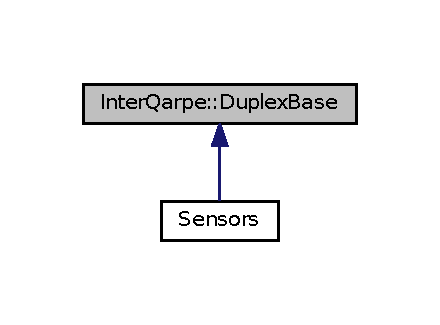
\includegraphics[width=211pt]{classInterQarpe_1_1DuplexBase__inherit__graph}
\end{center}
\end{figure}
\subsection*{Public Member Functions}
\begin{DoxyCompactItemize}
\item 
void \hyperlink{classInterQarpe_1_1DuplexBase_afd89e07392cc99212fa7fdaa5b4f1ca9}{routine} (void)
\begin{DoxyCompactList}\small\item\em Execute common task needed by the Inter\+Qarpe protocol to manage the connection. \end{DoxyCompactList}\item 
bool \hyperlink{classInterQarpe_1_1DuplexBase_a625debf26eb65849e398b46b26c4bb10}{is\+\_\+connected} (void)
\begin{DoxyCompactList}\small\item\em Check if we have we are connected to the other device. \end{DoxyCompactList}\item 
\hyperlink{classInterQarpe_1_1QueryResult}{Query\+Result} \hyperlink{classInterQarpe_1_1DuplexBase_a854f6b7c2a7a11bbd3e21b1db5cd8d6b}{query} (const char $\ast$query)
\begin{DoxyCompactList}\small\item\em Send a query to the other device. \end{DoxyCompactList}\end{DoxyCompactItemize}
\subsection*{Protected Member Functions}
\begin{DoxyCompactItemize}
\item 
{\footnotesize template$<$typename T $>$ }\\void \hyperlink{classInterQarpe_1_1DuplexBase_acf8055b4b74a31d87d2bb7f996bb70ad}{send\+\_\+response\+\_\+ok} (T $\ast$data)
\begin{DoxyCompactList}\small\item\em send a \char`\"{}ok\char`\"{} response to the other device \end{DoxyCompactList}\item 
{\footnotesize template$<$typename T $>$ }\\void \hyperlink{classInterQarpe_1_1DuplexBase_abb519576ef34c52b3f9f308ae8985fc4}{send\+\_\+response\+\_\+error} (T $\ast$data)
\begin{DoxyCompactList}\small\item\em send a \char`\"{}error\char`\"{} response to the other device \end{DoxyCompactList}\item 
\hypertarget{classInterQarpe_1_1DuplexBase_a897ceb69441859a534402332c366325f}{void \hyperlink{classInterQarpe_1_1DuplexBase_a897ceb69441859a534402332c366325f}{send\+\_\+badquery} (void)}\label{classInterQarpe_1_1DuplexBase_a897ceb69441859a534402332c366325f}

\begin{DoxyCompactList}\small\item\em Signal to the other side that the query is not handled on our side. \end{DoxyCompactList}\item 
\hypertarget{classInterQarpe_1_1DuplexBase_a0b2dc57b5951bd0d3a4b670ee860c496}{virtual void \hyperlink{classInterQarpe_1_1DuplexBase_a0b2dc57b5951bd0d3a4b670ee860c496}{on\+\_\+query} (const char $\ast$\hyperlink{classInterQarpe_1_1DuplexBase_a854f6b7c2a7a11bbd3e21b1db5cd8d6b}{query})}\label{classInterQarpe_1_1DuplexBase_a0b2dc57b5951bd0d3a4b670ee860c496}

\begin{DoxyCompactList}\small\item\em Hook that is called when a query is received. \end{DoxyCompactList}\end{DoxyCompactItemize}
\subsection*{Private Member Functions}
\begin{DoxyCompactItemize}
\item 
virtual int \hyperlink{classInterQarpe_1_1DuplexBase_a84945449769cfa079e543bcbad668b20}{write\+\_\+bytes} (uint8\+\_\+t $\ast$buf, size\+\_\+t count)=0
\begin{DoxyCompactList}\small\item\em Write bytes in the serial port. \end{DoxyCompactList}\item 
virtual int \hyperlink{classInterQarpe_1_1DuplexBase_ad66214fcff48f64165bcee960979e652}{read\+\_\+bytes} (uint8\+\_\+t $\ast$buf, size\+\_\+t count)=0
\begin{DoxyCompactList}\small\item\em Read \char`\"{}count\char`\"{} bytes from the serial port. \end{DoxyCompactList}\item 
virtual size\+\_\+t \hyperlink{classInterQarpe_1_1DuplexBase_a363d4fe7f3f058cd0622a26759bf7e17}{bytes\+\_\+available} (void)=0
\begin{DoxyCompactList}\small\item\em Return the number of bytes available on the serial port. \end{DoxyCompactList}\item 
virtual uint32\+\_\+t \hyperlink{classInterQarpe_1_1DuplexBase_a06cd56b01b03efb46597937de255406b}{now\+\_\+ms} (void)=0
\begin{DoxyCompactList}\small\item\em Return the time in milliseconds (used for timeout, so we don't care of the absolute value) \end{DoxyCompactList}\end{DoxyCompactItemize}


\subsection{Member Function Documentation}
\hypertarget{classInterQarpe_1_1DuplexBase_a363d4fe7f3f058cd0622a26759bf7e17}{\index{Inter\+Qarpe\+::\+Duplex\+Base@{Inter\+Qarpe\+::\+Duplex\+Base}!bytes\+\_\+available@{bytes\+\_\+available}}
\index{bytes\+\_\+available@{bytes\+\_\+available}!Inter\+Qarpe\+::\+Duplex\+Base@{Inter\+Qarpe\+::\+Duplex\+Base}}
\subsubsection[{bytes\+\_\+available}]{\setlength{\rightskip}{0pt plus 5cm}virtual size\+\_\+t Inter\+Qarpe\+::\+Duplex\+Base\+::bytes\+\_\+available (
\begin{DoxyParamCaption}
\item[{void}]{}
\end{DoxyParamCaption}
)\hspace{0.3cm}{\ttfamily [private]}, {\ttfamily [pure virtual]}}}\label{classInterQarpe_1_1DuplexBase_a363d4fe7f3f058cd0622a26759bf7e17}


Return the number of bytes available on the serial port. 

\begin{DoxyReturn}{Returns}
number of bytes available (if we can't get the value because of an error, we should return 0) 
\end{DoxyReturn}
\hypertarget{classInterQarpe_1_1DuplexBase_a625debf26eb65849e398b46b26c4bb10}{\index{Inter\+Qarpe\+::\+Duplex\+Base@{Inter\+Qarpe\+::\+Duplex\+Base}!is\+\_\+connected@{is\+\_\+connected}}
\index{is\+\_\+connected@{is\+\_\+connected}!Inter\+Qarpe\+::\+Duplex\+Base@{Inter\+Qarpe\+::\+Duplex\+Base}}
\subsubsection[{is\+\_\+connected}]{\setlength{\rightskip}{0pt plus 5cm}bool Inter\+Qarpe\+::\+Duplex\+Base\+::is\+\_\+connected (
\begin{DoxyParamCaption}
\item[{void}]{}
\end{DoxyParamCaption}
)}}\label{classInterQarpe_1_1DuplexBase_a625debf26eb65849e398b46b26c4bb10}


Check if we have we are connected to the other device. 

\begin{DoxyReturn}{Returns}
true if we have a valid connection with the other device 
\end{DoxyReturn}
\hypertarget{classInterQarpe_1_1DuplexBase_a06cd56b01b03efb46597937de255406b}{\index{Inter\+Qarpe\+::\+Duplex\+Base@{Inter\+Qarpe\+::\+Duplex\+Base}!now\+\_\+ms@{now\+\_\+ms}}
\index{now\+\_\+ms@{now\+\_\+ms}!Inter\+Qarpe\+::\+Duplex\+Base@{Inter\+Qarpe\+::\+Duplex\+Base}}
\subsubsection[{now\+\_\+ms}]{\setlength{\rightskip}{0pt plus 5cm}virtual uint32\+\_\+t Inter\+Qarpe\+::\+Duplex\+Base\+::now\+\_\+ms (
\begin{DoxyParamCaption}
\item[{void}]{}
\end{DoxyParamCaption}
)\hspace{0.3cm}{\ttfamily [private]}, {\ttfamily [pure virtual]}}}\label{classInterQarpe_1_1DuplexBase_a06cd56b01b03efb46597937de255406b}


Return the time in milliseconds (used for timeout, so we don't care of the absolute value) 

\begin{DoxyReturn}{Returns}
return the current time 
\end{DoxyReturn}
\hypertarget{classInterQarpe_1_1DuplexBase_a854f6b7c2a7a11bbd3e21b1db5cd8d6b}{\index{Inter\+Qarpe\+::\+Duplex\+Base@{Inter\+Qarpe\+::\+Duplex\+Base}!query@{query}}
\index{query@{query}!Inter\+Qarpe\+::\+Duplex\+Base@{Inter\+Qarpe\+::\+Duplex\+Base}}
\subsubsection[{query}]{\setlength{\rightskip}{0pt plus 5cm}{\bf Query\+Result} Inter\+Qarpe\+::\+Duplex\+Base\+::query (
\begin{DoxyParamCaption}
\item[{const char $\ast$}]{query}
\end{DoxyParamCaption}
)}}\label{classInterQarpe_1_1DuplexBase_a854f6b7c2a7a11bbd3e21b1db5cd8d6b}


Send a query to the other device. 

This function is blocking and will only return when we have a proper response to return (a.\+k.\+a response from the other device or timeout after the default duration without a response)


\begin{DoxyParams}{Parameters}
{\em query} & the query must be a 0-\/terminated string\\
\hline
\end{DoxyParams}
\begin{DoxyReturn}{Returns}
the query's result 
\end{DoxyReturn}
\hypertarget{classInterQarpe_1_1DuplexBase_ad66214fcff48f64165bcee960979e652}{\index{Inter\+Qarpe\+::\+Duplex\+Base@{Inter\+Qarpe\+::\+Duplex\+Base}!read\+\_\+bytes@{read\+\_\+bytes}}
\index{read\+\_\+bytes@{read\+\_\+bytes}!Inter\+Qarpe\+::\+Duplex\+Base@{Inter\+Qarpe\+::\+Duplex\+Base}}
\subsubsection[{read\+\_\+bytes}]{\setlength{\rightskip}{0pt plus 5cm}virtual int Inter\+Qarpe\+::\+Duplex\+Base\+::read\+\_\+bytes (
\begin{DoxyParamCaption}
\item[{uint8\+\_\+t $\ast$}]{buf, }
\item[{size\+\_\+t}]{count}
\end{DoxyParamCaption}
)\hspace{0.3cm}{\ttfamily [private]}, {\ttfamily [pure virtual]}}}\label{classInterQarpe_1_1DuplexBase_ad66214fcff48f64165bcee960979e652}


Read \char`\"{}count\char`\"{} bytes from the serial port. 

If less bytes are available this function will not wait for the missing bytes and return


\begin{DoxyParams}{Parameters}
{\em buf} & pointer to a buffer of \char`\"{}count\char`\"{} bytes that will be overwritten \\
\hline
{\em count} & number of bytes to read from the serial port\\
\hline
\end{DoxyParams}
\begin{DoxyReturn}{Returns}
number of bytes read successfully from the serial port (can be less than \char`\"{}count\char`\"{}) or -\/1 if an error occur and exception are disabled. 
\end{DoxyReturn}
\hypertarget{classInterQarpe_1_1DuplexBase_afd89e07392cc99212fa7fdaa5b4f1ca9}{\index{Inter\+Qarpe\+::\+Duplex\+Base@{Inter\+Qarpe\+::\+Duplex\+Base}!routine@{routine}}
\index{routine@{routine}!Inter\+Qarpe\+::\+Duplex\+Base@{Inter\+Qarpe\+::\+Duplex\+Base}}
\subsubsection[{routine}]{\setlength{\rightskip}{0pt plus 5cm}void Inter\+Qarpe\+::\+Duplex\+Base\+::routine (
\begin{DoxyParamCaption}
\item[{void}]{}
\end{DoxyParamCaption}
)}}\label{classInterQarpe_1_1DuplexBase_afd89e07392cc99212fa7fdaa5b4f1ca9}


Execute common task needed by the Inter\+Qarpe protocol to manage the connection. 

This function must be executed in order to receive packet. You may want to execute it in each iteration of your main loop. \hypertarget{classInterQarpe_1_1DuplexBase_abb519576ef34c52b3f9f308ae8985fc4}{\index{Inter\+Qarpe\+::\+Duplex\+Base@{Inter\+Qarpe\+::\+Duplex\+Base}!send\+\_\+response\+\_\+error@{send\+\_\+response\+\_\+error}}
\index{send\+\_\+response\+\_\+error@{send\+\_\+response\+\_\+error}!Inter\+Qarpe\+::\+Duplex\+Base@{Inter\+Qarpe\+::\+Duplex\+Base}}
\subsubsection[{send\+\_\+response\+\_\+error}]{\setlength{\rightskip}{0pt plus 5cm}template$<$typename T $>$ void Inter\+Qarpe\+::\+Duplex\+Base\+::send\+\_\+response\+\_\+error (
\begin{DoxyParamCaption}
\item[{T $\ast$}]{data}
\end{DoxyParamCaption}
)\hspace{0.3cm}{\ttfamily [protected]}}}\label{classInterQarpe_1_1DuplexBase_abb519576ef34c52b3f9f308ae8985fc4}


send a \char`\"{}error\char`\"{} response to the other device 


\begin{DoxyTemplParams}{Template Parameters}
{\em T} & type of data to send \\
\hline
\end{DoxyTemplParams}
\hypertarget{classInterQarpe_1_1DuplexBase_acf8055b4b74a31d87d2bb7f996bb70ad}{\index{Inter\+Qarpe\+::\+Duplex\+Base@{Inter\+Qarpe\+::\+Duplex\+Base}!send\+\_\+response\+\_\+ok@{send\+\_\+response\+\_\+ok}}
\index{send\+\_\+response\+\_\+ok@{send\+\_\+response\+\_\+ok}!Inter\+Qarpe\+::\+Duplex\+Base@{Inter\+Qarpe\+::\+Duplex\+Base}}
\subsubsection[{send\+\_\+response\+\_\+ok}]{\setlength{\rightskip}{0pt plus 5cm}template$<$typename T $>$ void Inter\+Qarpe\+::\+Duplex\+Base\+::send\+\_\+response\+\_\+ok (
\begin{DoxyParamCaption}
\item[{T $\ast$}]{data}
\end{DoxyParamCaption}
)\hspace{0.3cm}{\ttfamily [protected]}}}\label{classInterQarpe_1_1DuplexBase_acf8055b4b74a31d87d2bb7f996bb70ad}


send a \char`\"{}ok\char`\"{} response to the other device 


\begin{DoxyTemplParams}{Template Parameters}
{\em T} & type of data to send \\
\hline
\end{DoxyTemplParams}
\hypertarget{classInterQarpe_1_1DuplexBase_a84945449769cfa079e543bcbad668b20}{\index{Inter\+Qarpe\+::\+Duplex\+Base@{Inter\+Qarpe\+::\+Duplex\+Base}!write\+\_\+bytes@{write\+\_\+bytes}}
\index{write\+\_\+bytes@{write\+\_\+bytes}!Inter\+Qarpe\+::\+Duplex\+Base@{Inter\+Qarpe\+::\+Duplex\+Base}}
\subsubsection[{write\+\_\+bytes}]{\setlength{\rightskip}{0pt plus 5cm}virtual int Inter\+Qarpe\+::\+Duplex\+Base\+::write\+\_\+bytes (
\begin{DoxyParamCaption}
\item[{uint8\+\_\+t $\ast$}]{buf, }
\item[{size\+\_\+t}]{count}
\end{DoxyParamCaption}
)\hspace{0.3cm}{\ttfamily [private]}, {\ttfamily [pure virtual]}}}\label{classInterQarpe_1_1DuplexBase_a84945449769cfa079e543bcbad668b20}


Write bytes in the serial port. 


\begin{DoxyParams}{Parameters}
{\em buf} & pointer to \char`\"{}count\char`\"{} bytes that will be send through the serial port \\
\hline
{\em count} & number of bytes to be sent\\
\hline
\end{DoxyParams}
\begin{DoxyReturn}{Returns}
number of bytes written succesfully or -\/1 if we failed to write altogether and exception are disabled 
\end{DoxyReturn}


The documentation for this class was generated from the following file\+:\begin{DoxyCompactItemize}
\item 
include/Inter\+Qarpe.\+h\end{DoxyCompactItemize}

\hypertarget{classInterQarpe_1_1QueryResult}{\section{Inter\+Qarpe\+:\+:Query\+Result Class Reference}
\label{classInterQarpe_1_1QueryResult}\index{Inter\+Qarpe\+::\+Query\+Result@{Inter\+Qarpe\+::\+Query\+Result}}
}


Represent the result of a query.  




{\ttfamily \#include $<$Query\+Result.\+h$>$}

\subsection*{Public Types}
\begin{DoxyCompactItemize}
\item 
enum \hyperlink{classInterQarpe_1_1QueryResult_ad265093e5dea69f229df989d4e18cbb4}{result\+\_\+t} \{ {\bfseries R\+E\+S\+P\+O\+N\+S\+E\+\_\+\+O\+K}, 
{\bfseries R\+E\+S\+P\+O\+N\+S\+E\+\_\+\+E\+R\+R\+O\+R}, 
{\bfseries B\+A\+D\+\_\+\+Q\+U\+E\+R\+Y}, 
{\bfseries T\+I\+M\+E\+O\+U\+T}
 \}
\begin{DoxyCompactList}\small\item\em Different results a query can take\+: \end{DoxyCompactList}\end{DoxyCompactItemize}
\subsection*{Public Member Functions}
\begin{DoxyCompactItemize}
\item 
\hyperlink{classInterQarpe_1_1QueryResult_aeaa273884f3d8494f3451ef1da3afcba}{Query\+Result} (\hyperlink{classInterQarpe_1_1QueryResult_ad265093e5dea69f229df989d4e18cbb4}{result\+\_\+t} status, uint8\+\_\+t $\ast$data, size\+\_\+t data\+\_\+size)
\begin{DoxyCompactList}\small\item\em Constructor of \hyperlink{classInterQarpe_1_1QueryResult}{Query\+Result}. \end{DoxyCompactList}\item 
\hyperlink{classInterQarpe_1_1QueryResult_ad265093e5dea69f229df989d4e18cbb4}{result\+\_\+t} \hyperlink{classInterQarpe_1_1QueryResult_a08d4addcab59886e2e76f1028fe3ff9b}{get\+\_\+result} (void)
\begin{DoxyCompactList}\small\item\em Return the current status of the query. \end{DoxyCompactList}\item 
{\footnotesize template$<$typename T $>$ }\\bool \hyperlink{classInterQarpe_1_1QueryResult_a2a128d20e11bf7118844c73ec2035c76}{get\+\_\+data} (T $\ast$data)
\begin{DoxyCompactList}\small\item\em Return data received from the other device. \end{DoxyCompactList}\end{DoxyCompactItemize}


\subsection{Detailed Description}
Represent the result of a query. 


\begin{DoxyTemplParams}{Template Parameters}
{\em T} & represent the data the query should \\
\hline
\end{DoxyTemplParams}


\subsection{Member Enumeration Documentation}
\hypertarget{classInterQarpe_1_1QueryResult_ad265093e5dea69f229df989d4e18cbb4}{\index{Inter\+Qarpe\+::\+Query\+Result@{Inter\+Qarpe\+::\+Query\+Result}!result\+\_\+t@{result\+\_\+t}}
\index{result\+\_\+t@{result\+\_\+t}!Inter\+Qarpe\+::\+Query\+Result@{Inter\+Qarpe\+::\+Query\+Result}}
\subsubsection[{result\+\_\+t}]{\setlength{\rightskip}{0pt plus 5cm}enum {\bf Inter\+Qarpe\+::\+Query\+Result\+::result\+\_\+t}}}\label{classInterQarpe_1_1QueryResult_ad265093e5dea69f229df989d4e18cbb4}


Different results a query can take\+: 


\begin{DoxyItemize}
\item R\+E\+S\+P\+O\+N\+S\+E\+\_\+\mbox{[}O\+K$\vert$\+E\+R\+R\+O\+R\mbox{]}\+: Positive/negative response from the other device.
\item B\+A\+D\+\_\+\+Q\+U\+E\+R\+Y\+: Error received from the other device.
\item T\+I\+M\+E\+O\+U\+T\+: No response from the other device. 
\end{DoxyItemize}

\subsection{Constructor \& Destructor Documentation}
\hypertarget{classInterQarpe_1_1QueryResult_aeaa273884f3d8494f3451ef1da3afcba}{\index{Inter\+Qarpe\+::\+Query\+Result@{Inter\+Qarpe\+::\+Query\+Result}!Query\+Result@{Query\+Result}}
\index{Query\+Result@{Query\+Result}!Inter\+Qarpe\+::\+Query\+Result@{Inter\+Qarpe\+::\+Query\+Result}}
\subsubsection[{Query\+Result}]{\setlength{\rightskip}{0pt plus 5cm}Inter\+Qarpe\+::\+Query\+Result\+::\+Query\+Result (
\begin{DoxyParamCaption}
\item[{{\bf Query\+Result\+::result\+\_\+t}}]{result, }
\item[{uint8\+\_\+t $\ast$}]{data, }
\item[{size\+\_\+t}]{data\+\_\+size}
\end{DoxyParamCaption}
)}}\label{classInterQarpe_1_1QueryResult_aeaa273884f3d8494f3451ef1da3afcba}


Constructor of \hyperlink{classInterQarpe_1_1QueryResult}{Query\+Result}. 


\begin{DoxyParams}{Parameters}
{\em result} & of the query \\
\hline
{\em data} & a pointer to the data \\
\hline
{\em data\+\_\+size} & number of bytes available in the data buffer \\
\hline
\end{DoxyParams}


\subsection{Member Function Documentation}
\hypertarget{classInterQarpe_1_1QueryResult_a2a128d20e11bf7118844c73ec2035c76}{\index{Inter\+Qarpe\+::\+Query\+Result@{Inter\+Qarpe\+::\+Query\+Result}!get\+\_\+data@{get\+\_\+data}}
\index{get\+\_\+data@{get\+\_\+data}!Inter\+Qarpe\+::\+Query\+Result@{Inter\+Qarpe\+::\+Query\+Result}}
\subsubsection[{get\+\_\+data}]{\setlength{\rightskip}{0pt plus 5cm}template$<$typename T $>$ bool Inter\+Qarpe\+::\+Query\+Result\+::get\+\_\+data (
\begin{DoxyParamCaption}
\item[{T $\ast$}]{data}
\end{DoxyParamCaption}
)}}\label{classInterQarpe_1_1QueryResult_a2a128d20e11bf7118844c73ec2035c76}


Return data received from the other device. 


\begin{DoxyParams}{Parameters}
{\em data} & will be returned through this pointer if any \\
\hline
\end{DoxyParams}

\begin{DoxyTemplParams}{Template Parameters}
{\em T} & type of data that will be returned\\
\hline
\end{DoxyTemplParams}
\begin{DoxyReturn}{Returns}
true if we were able do recover enough data to build a T 
\end{DoxyReturn}
\hypertarget{classInterQarpe_1_1QueryResult_a08d4addcab59886e2e76f1028fe3ff9b}{\index{Inter\+Qarpe\+::\+Query\+Result@{Inter\+Qarpe\+::\+Query\+Result}!get\+\_\+result@{get\+\_\+result}}
\index{get\+\_\+result@{get\+\_\+result}!Inter\+Qarpe\+::\+Query\+Result@{Inter\+Qarpe\+::\+Query\+Result}}
\subsubsection[{get\+\_\+result}]{\setlength{\rightskip}{0pt plus 5cm}{\bf Query\+Result\+::result\+\_\+t} Inter\+Qarpe\+::\+Query\+Result\+::get\+\_\+result (
\begin{DoxyParamCaption}
\item[{void}]{}
\end{DoxyParamCaption}
)}}\label{classInterQarpe_1_1QueryResult_a08d4addcab59886e2e76f1028fe3ff9b}


Return the current status of the query. 

\begin{DoxyReturn}{Returns}
result of query 
\end{DoxyReturn}


The documentation for this class was generated from the following file\+:\begin{DoxyCompactItemize}
\item 
include/Query\+Result.\+h\end{DoxyCompactItemize}

\hypertarget{classSensors}{\section{Sensors Class Reference}
\label{classSensors}\index{Sensors@{Sensors}}
}


Inheritance diagram for Sensors\+:\nopagebreak
\begin{figure}[H]
\begin{center}
\leavevmode
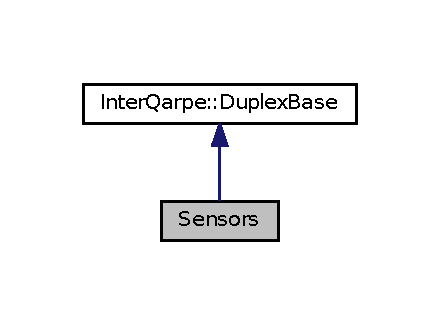
\includegraphics[width=211pt]{classSensors__inherit__graph}
\end{center}
\end{figure}


Collaboration diagram for Sensors\+:\nopagebreak
\begin{figure}[H]
\begin{center}
\leavevmode
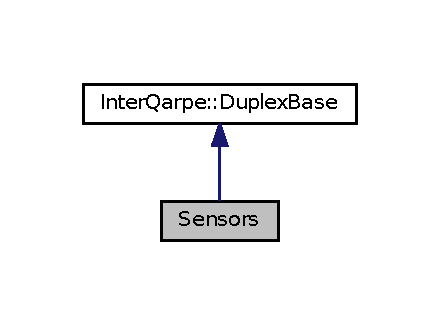
\includegraphics[width=211pt]{classSensors__coll__graph}
\end{center}
\end{figure}
\subsection*{Public Member Functions}
\begin{DoxyCompactItemize}
\item 
bool \hyperlink{classSensors_a6405f7378789aba2b97a178fa7d70dc8}{open\+\_\+port} (const char $\ast$port)
\begin{DoxyCompactList}\small\item\em Open a port (e.\+g /dev/tty\+S0 on Linux, C\+O\+M1 on Windows etc.) \end{DoxyCompactList}\item 
bool \hyperlink{classSensors_ad24b2e04c9190324a204c0f9881df004}{close\+\_\+port} ()
\begin{DoxyCompactList}\small\item\em Close the current port. \end{DoxyCompactList}\end{DoxyCompactItemize}
\subsection*{Additional Inherited Members}


\subsection{Member Function Documentation}
\hypertarget{classSensors_ad24b2e04c9190324a204c0f9881df004}{\index{Sensors@{Sensors}!close\+\_\+port@{close\+\_\+port}}
\index{close\+\_\+port@{close\+\_\+port}!Sensors@{Sensors}}
\subsubsection[{close\+\_\+port}]{\setlength{\rightskip}{0pt plus 5cm}bool Sensors\+::close\+\_\+port (
\begin{DoxyParamCaption}
{}
\end{DoxyParamCaption}
)\hspace{0.3cm}{\ttfamily [inline]}}}\label{classSensors_ad24b2e04c9190324a204c0f9881df004}


Close the current port. 

If it's not opened, we return -\/1. If an error occur while closing the port, we return -\/1 as well. The Linux kernel assure us that close will always free the descriptor. errno will be said on case of an error.

\begin{DoxyReturn}{Returns}
true if we succesfully closed the current file descriptor with no error 
\end{DoxyReturn}
\hypertarget{classSensors_a6405f7378789aba2b97a178fa7d70dc8}{\index{Sensors@{Sensors}!open\+\_\+port@{open\+\_\+port}}
\index{open\+\_\+port@{open\+\_\+port}!Sensors@{Sensors}}
\subsubsection[{open\+\_\+port}]{\setlength{\rightskip}{0pt plus 5cm}bool Sensors\+::open\+\_\+port (
\begin{DoxyParamCaption}
\item[{const char $\ast$}]{port}
\end{DoxyParamCaption}
)\hspace{0.3cm}{\ttfamily [inline]}}}\label{classSensors_a6405f7378789aba2b97a178fa7d70dc8}


Open a port (e.\+g /dev/tty\+S0 on Linux, C\+O\+M1 on Windows etc.) 


\begin{DoxyParams}{Parameters}
{\em port} & port designation\\
\hline
\end{DoxyParams}
\begin{DoxyReturn}{Returns}
true if the port was succesfully opened 
\end{DoxyReturn}


The documentation for this class was generated from the following file\+:\begin{DoxyCompactItemize}
\item 
include/Sensors.\+h\end{DoxyCompactItemize}

\hypertarget{classSensorsDatabase}{\section{Sensors\+Database Class Reference}
\label{classSensorsDatabase}\index{Sensors\+Database@{Sensors\+Database}}
}
\subsection*{Public Member Functions}
\begin{DoxyCompactItemize}
\item 
\hypertarget{classSensorsDatabase_a0f4f373b6b431d393965b96d34271863}{{\bfseries Sensors\+Database} (const char $\ast$path)}\label{classSensorsDatabase_a0f4f373b6b431d393965b96d34271863}

\item 
\hypertarget{classSensorsDatabase_a40a8126a616bd6933d4fabff016d3eb4}{void \hyperlink{classSensorsDatabase_a40a8126a616bd6933d4fabff016d3eb4}{insert\+\_\+poll} (time\+\_\+t created)}\label{classSensorsDatabase_a40a8126a616bd6933d4fabff016d3eb4}

\begin{DoxyCompactList}\small\item\em Insert a new poll in the database. \end{DoxyCompactList}\end{DoxyCompactItemize}
\subsection*{Private Member Functions}
\begin{DoxyCompactItemize}
\item 
\hypertarget{classSensorsDatabase_aa5e16408e6283c1bb307cc0d2ea6ee29}{sqlite3 $\ast$ {\bfseries open\+\_\+database} ()}\label{classSensorsDatabase_aa5e16408e6283c1bb307cc0d2ea6ee29}

\item 
\hypertarget{classSensorsDatabase_a4b57d4c939653a74515e372653065f5f}{bool {\bfseries configure\+\_\+database} ()}\label{classSensorsDatabase_a4b57d4c939653a74515e372653065f5f}

\end{DoxyCompactItemize}
\subsection*{Private Attributes}
\begin{DoxyCompactItemize}
\item 
\hypertarget{classSensorsDatabase_a18cf8a737f550d5028f21c10b26b8ffe}{sqlite3 $\ast$ {\bfseries db}}\label{classSensorsDatabase_a18cf8a737f550d5028f21c10b26b8ffe}

\end{DoxyCompactItemize}


The documentation for this class was generated from the following file\+:\begin{DoxyCompactItemize}
\item 
include/Sensors\+Database.\+h\end{DoxyCompactItemize}

%--- End generated contents ---

% Index
\newpage
\phantomsection
\addcontentsline{toc}{chapter}{Index}
\printindex

\end{document}
